\section{Développement}
%-------------------------------------------------------------------------------------------------------------------------
\subsection{Installation}
A mon arrivé à l'entreprise, une visite guidée était primordial afin de me familiariser avec le milieu du travail, de faire connaissance avec les futures collègues également. Après cela, on passe à notre poste de travail pour faire le point sur tous les outils mis à ma disposition (PC, 2 écrans, souris, clavier, etc.). Ainsi, une installation de l'environnement de travail et obligatoire, car la machine reçue ne contient qu'un système d’exploitation Windows (qu'on peut rien faire avec).\\
Donc j'ai réalisé les tâches suivantes :
\begin{itemize}
	\item Installation d'Ubuntu 18.04.
	\item Installation d'OpenJDK, Python, PIP, GCC, etc.  
	\item Installation d'Intellij idea (éditeur java).
	\item Installation de Pycharm (éditeur Python).
	\item Installation de Maven.
	\item Installation de Postman.
	\item Configuration des variable global JAVA{\_}HOME, etc.
	\item Installation et configuration du client Barracuda VPN.
\end{itemize}
%-------------------------------------------------------------------------------------------------------------------------
\subsection{Training}
Avant de m'initier vraiment dans le vif du sujet de mon stage, j'ai commencé par faire des petits exercices dans le but de m'adapter et de me familiariser avec la méthode de travail de l'équipe back-end. Ces exercices avaient pour but de m'aider à me familiariser avec la manière du développement de l'équipe, parmi ces exercices :
\begin{itemize}
\item GitLab :
	\begin{itemize}
		\item "Fork" le projet.
		\item "Clone" le projet.
		\item Travailler sur une branche "develop".
		\item Faire des modifications on faisant des commits régulièrement, pour garder des traces.
		\item Squash les commits avec leurs façon.
		\item Poussé le code à la fin.
		\item "Merge request" pour un développeur senior.
	\end{itemize}
\item Java :
	\begin{itemize}
		\item Création et configuration d'un projet maven.
		\item Gérer les plugins et les dépendances nécessaire.
		\item Coder des exercices sur la notion de "marshalling" et "unmarshalling".
		\item Travailler sur une première facture au format JSON(JSON $\to$ java et java $\to$ JSON).
	\end{itemize}
\item Python :
	\begin{itemize}
		\item Les modules, les packages, les classes,		
		\item La notion de "marshalling" et "unmarshalling".
	\end{itemize}
\end{itemize} 
%-------------------------------------------------------------------------------------------------------------------------
\subsection{b2b-Enedis (Java)}
\begin{center}
	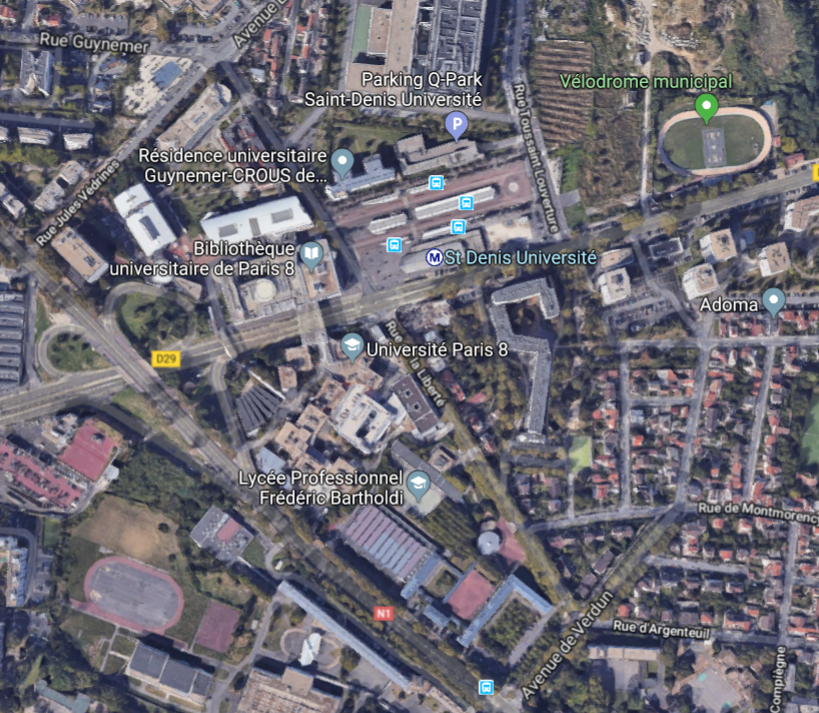
\includegraphics[scale=0.2]{4.png}
	\captionof{figure}{schéma explicatif de b2b-Enedis}
\end{center}
\subsubsection{Introduction}
Ce projet consiste à implémenter un traducteur de données techniques et contractuelles (DTC) d'Enedis vers des "meter" Energisme. Le projet est né d'un besoin de récupérer des données qui figurent sur ces DTC, afin de préparer ces données et de réaliser des courbes ou des graphes des puissances souscrites.\\
Les détails nécessaires afin de réaliser le traducteur figure sur un ticket JIRA, qui exprime le besoin, le résultat attendu et le mapping qu'il faut faire. De façon plus semple :
\begin{itemize}
	\item Les données : des DTC (données technique et contractuelle) fournies par Enedis au format XML dans leur API.
	\item Le traducteur : notre traducteur va récupérer les informations  nécessaires des fichiers XML.
	\item Le résultat : les informations récupérées seront mises dans des objet "meter" après dans des fichiers JSON, selon un format de l'entreprise.
\end{itemize}


Ma tâche consisté à travailler sur le carré vert "le traducteur". Alors j'ai procédé de la manière qu'on voit sur la \emph{figure 2}.
%-------------------------------------------------------------------------------------------------------------------------
\subsubsection{Implémentation}
Ce projet contient 4 packages essentiels(unmarshalling, meter, mapping et types) et une classe principale main, la \emph{figure 2} représente à schéma explicatif, voilà l'utilité de chaque composante : 
\begin{center}
	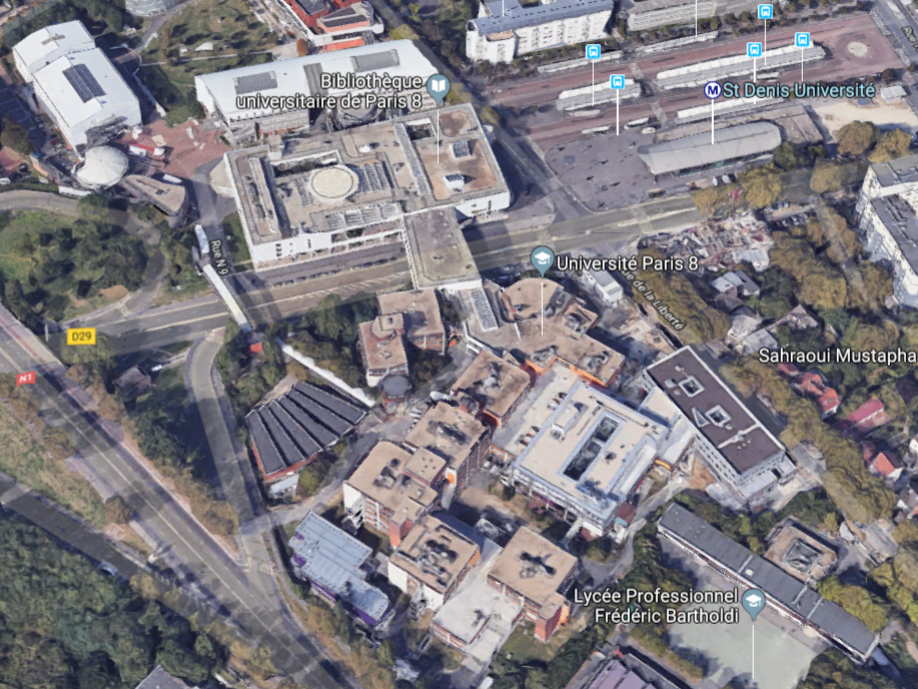
\includegraphics[scale=0.45]{5.png}
	 \captionof{figure}{Architecture du traducteur}
\end{center}
%========================================= class main
\textbf{Classe main :} c'est la classe principale qui prend les données d'entrée (les DTC) sous forme de répertoire qui les contient. 
Notre main reçoit deux arguments, le dossier source (qui contient les DTC au format XML) et le dossier de destination (qui va contenir les meters au format JSON).\\
\begin{center}
	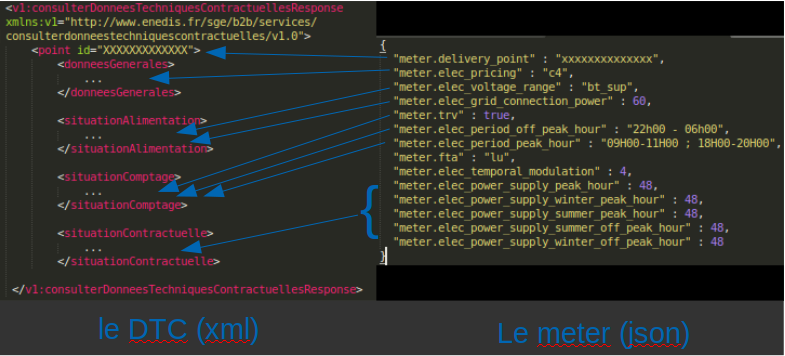
\includegraphics[scale=0.35]{13.png}
 	\captionof{figure}{DTC vs Meter}
\end{center}
Elle contient aussi une méthode "translateDTC" qui prend les deux arguments si dessus et réalise les opérations suivantes sur tous les DTC :
\begin{itemize}
	\item "unmarshaling" (fichier XML $\to$ objet JAVA).
	\item traduction de l'objet java avec le bon mapping vers un autre objet java (objet JAVA $\to$ objet JAVA).
	\item "marshalling" (objet java $\to$ fichier JSON).	
\end{itemize}
\begin{center}
	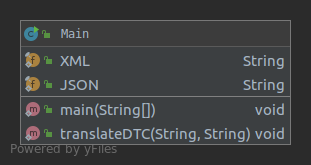
\includegraphics[scale=0.5]{6.png}
	\captionof{figure}{Diagramme de classe de Main}
\end{center}
%========================================= package unmarshalling
\textbf{Package unmarshalling :} ce package contient deux classes qui nous permet de faire :
\begin{itemize}
	\item fichier XML $\to$ objet JAVA
	\item objet JAVA $\to$ fichier JSON
\end{itemize}
\begin{center}
	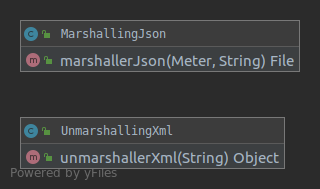
\includegraphics[scale=0.5]{8.png}
	\captionof{figure}{diagramme de classe explicatif du package unmarshalling}
\end{center}
%========================================= package types	
\textbf{Package types :} ce package contient toutes les classes généré grâce à un outil qui s'appelle "xjc" de JAXB, cette commande permet de générer un jeu de classes à l'aide d'un schéma xsd. Le schéma utilisé afin de générer ces classes est composé de plusieurs documents XSD fourni par Enedis, ces documents permettant de définir la structure et le type de contenu de leurs documents XML (les DTC).\\
Pour l'utilisation de cette commande, il suffit de taper en ligne de commande : xjc -p nomDuPackage schema.xsd\\
Grâce à ces classes générées, on peut faire de l'unmarshalling, c'est-à-dire avoir un objet java pour un fichier XML.
\begin{center}
	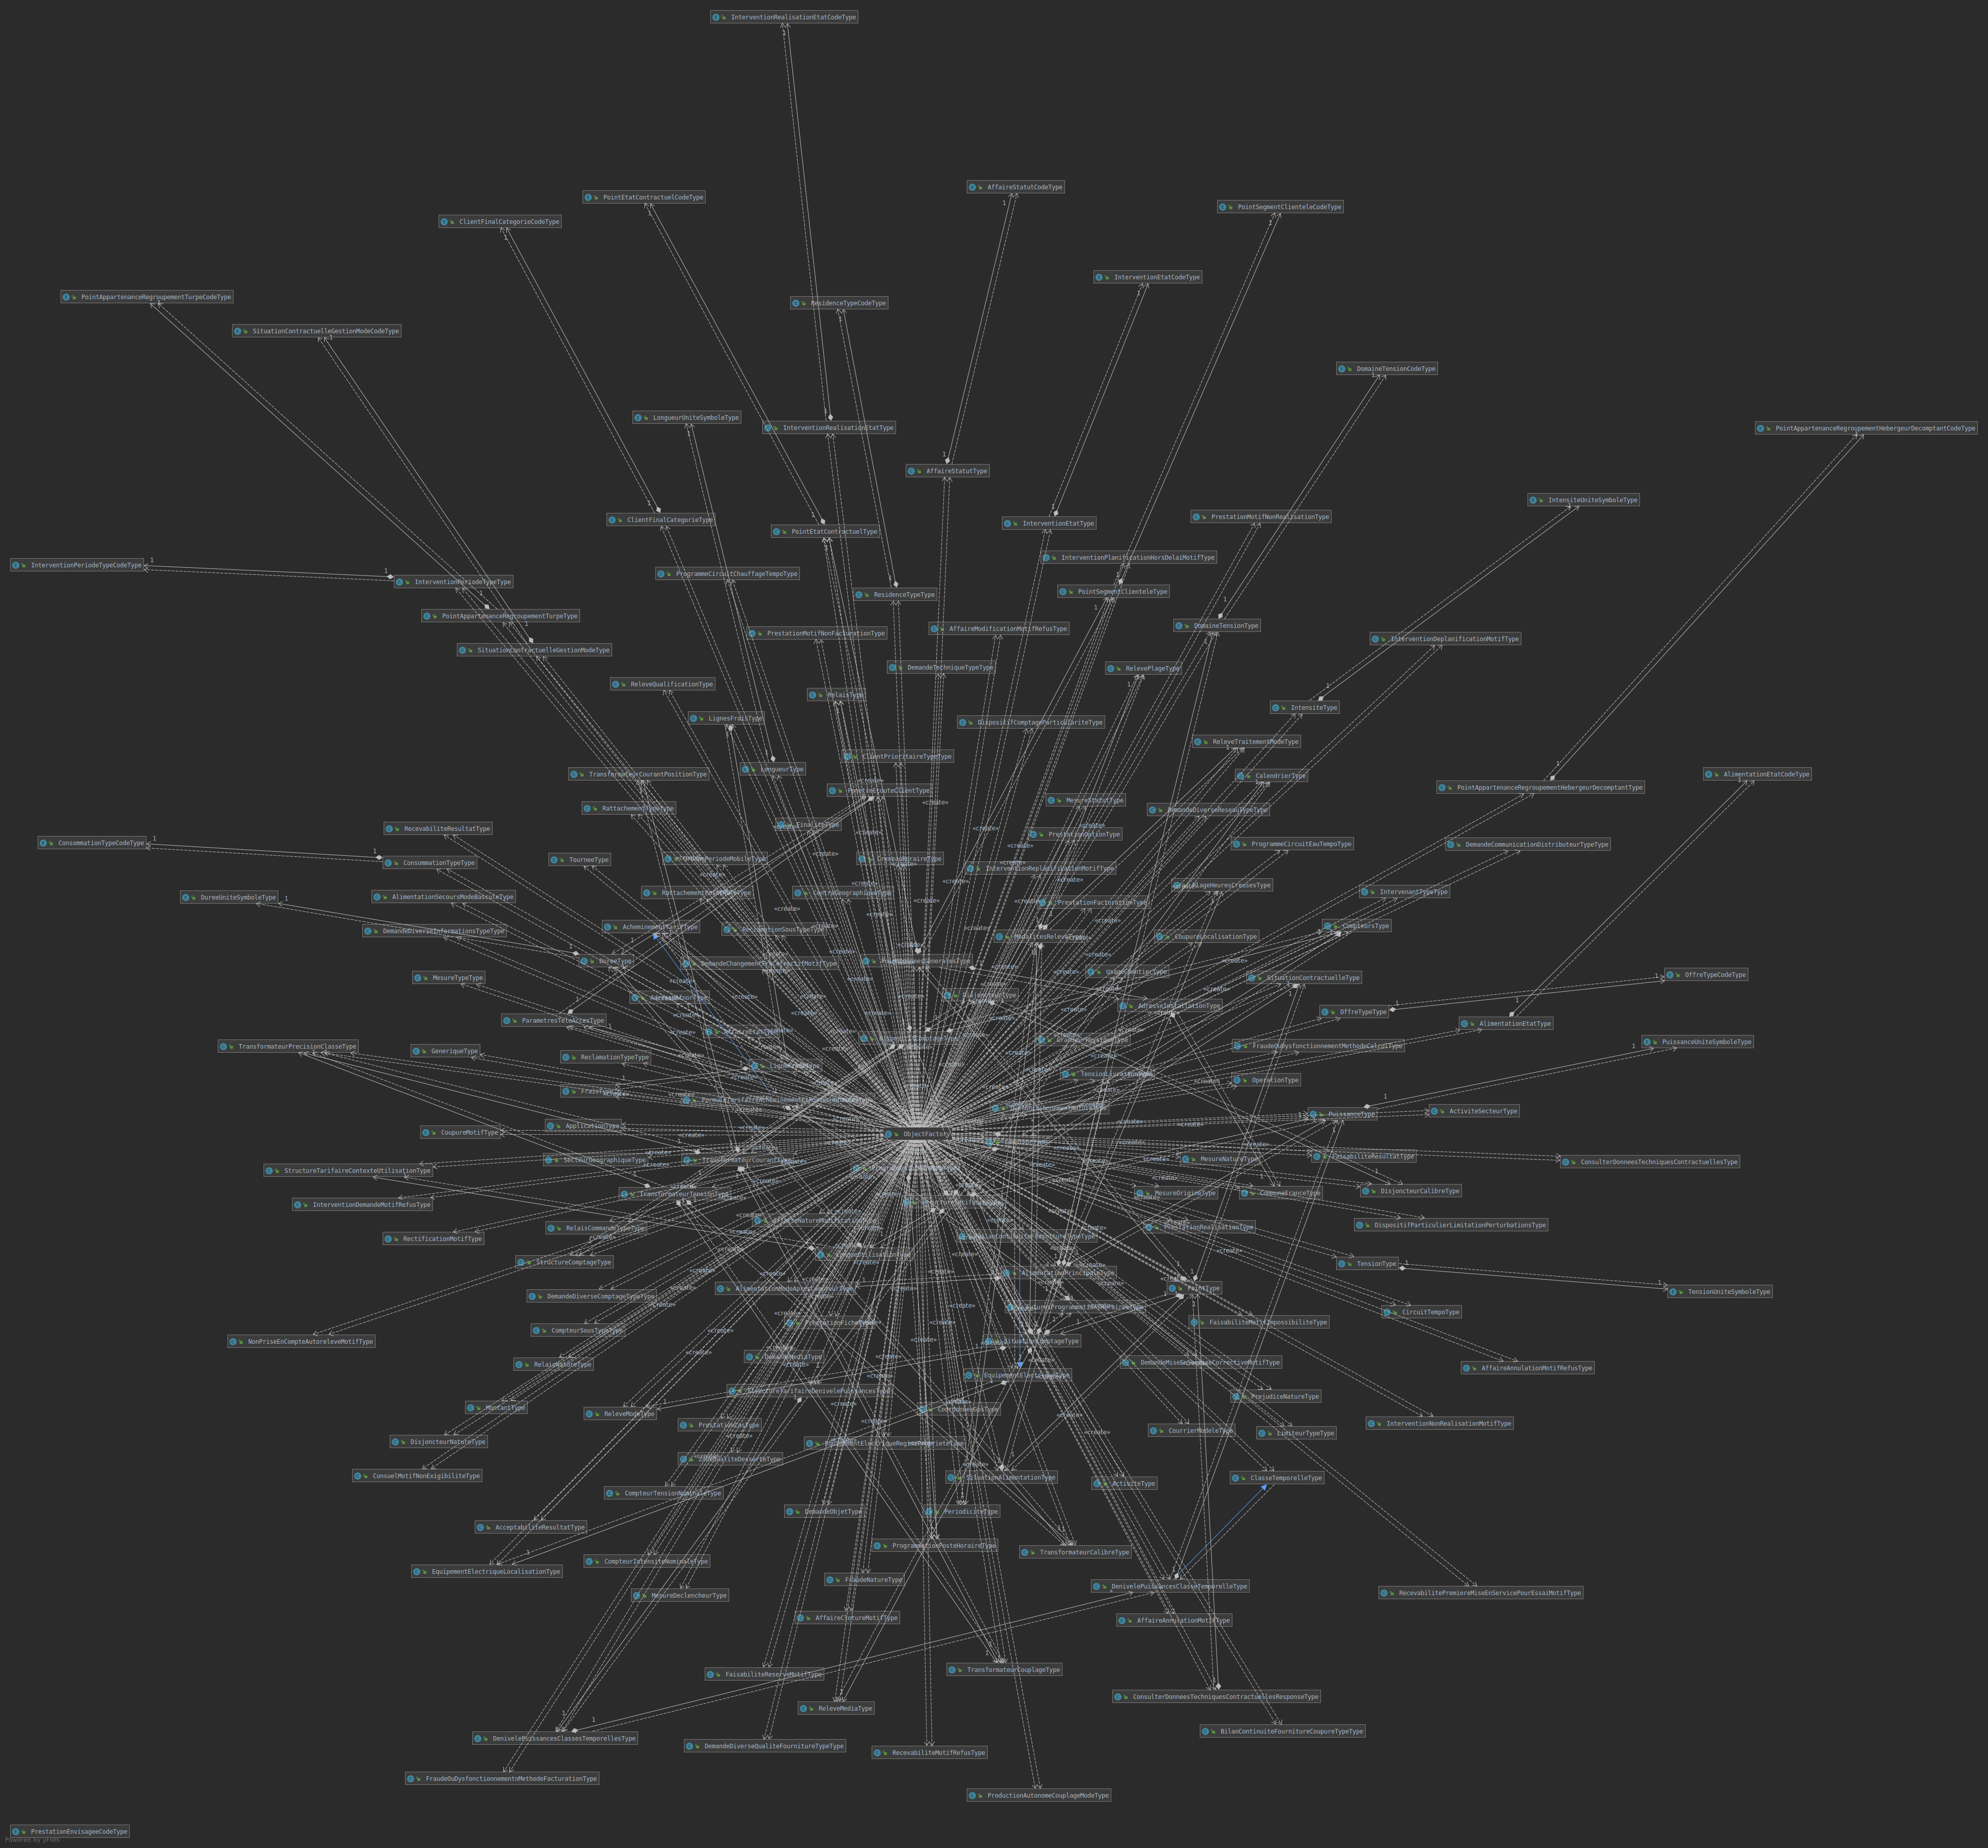
\includegraphics[scale=0.05]{9.png}
	\captionof{figure}{diagramme de classe explicatif du package types, 187 classes générer}
\end{center}	
%========================================= package meter
\textbf{Package meter :} contient la classe Meter.java, qui représente l'objet java qui va devenir le fichier JSON. Cette classe contient tous les noms de clés que peut avoir le fichier JSON et une Map qui va contenir des clés et leurs valeurs d'une instance de cette classe. 		
\begin{center}
	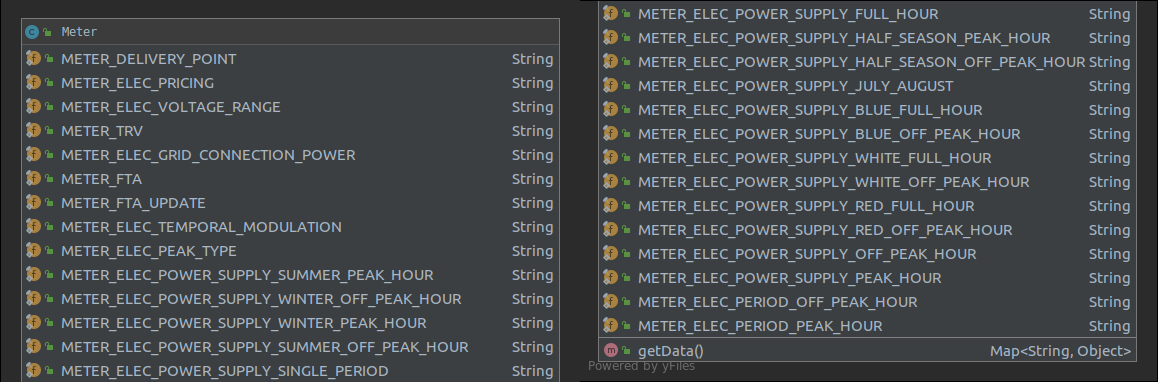
\includegraphics[scale=1]{10.png}
	\captionof{figure}{diagramme de classe de Meter.java}
\end{center}	
%========================================= package mapping
\textbf{Package mapping :} ce package contient toutes les classes nécessaire à la traduction et au mapping qu'il faut réaliser.
\begin{center}
	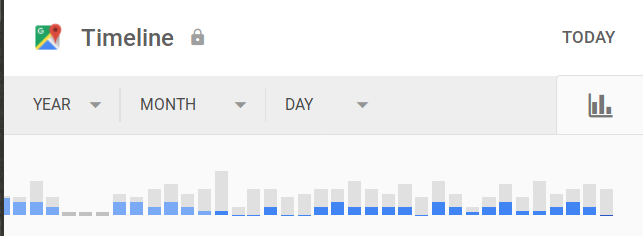
\includegraphics[scale=0.5]{7.png}
	\captionof{figure}{diagramme de classe explicatif du package mapping}
\end{center}
Il contient 3 classes principales :
\begin{itemize}
	\item TranslatorDTC : 
		\begin{center}
			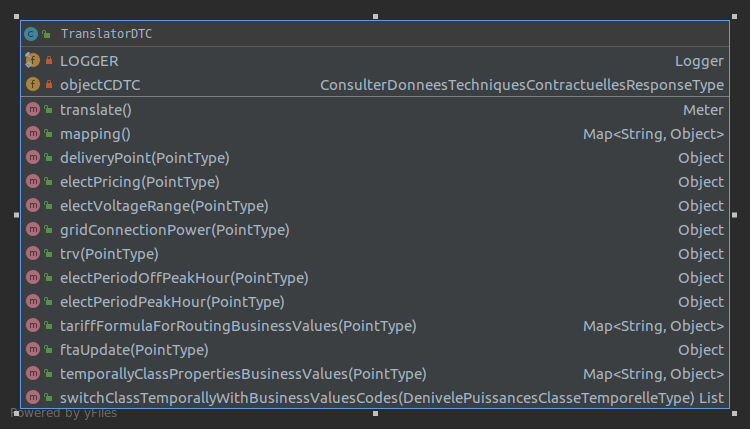
\includegraphics[scale=0.3]{11.png}
			\captionof{figure}{diagramme de classe de TranslatorDTC.java}
		\end{center}
		Cette classe, elle s’occupe de la traduction, ce qui veut dire récupérer de telles valeurs d'un objet java (ConsultationDonneesTechniquesContractuellesResponseType) et les placer dans de tels champs dans un autre objet java (meter), on respecte certain règles.
		
		
		Il y a deux méthodes principales "translate" et  "mapping" ainsi que d'autres méthodes :
		\begin{itemize}
			\item "mapping" : renvoi une Map qui contient tous les champs à récupérer dans l'objet qui représente le fichier XML (CDTC), pour chaque clé de la Map on lui associer la valeur trouvée dans le fichier XML sinon on lui associer un null.
			\item "translate" : renvoi un objet Meter initialisé avec la Map que renvoi "mapping" en filtrant tous les valeurs null, donc on garde une Map qui contient les valeurs trouvent dans le (CDTC).
			\item les autres méthodes chacune récupérer une valeur dans l'objet (CDTC) associer à un champ qui porte presque le même nom que la méthode, par ailleurs d'autres méthodes récupèrent une Map de clé et valeur, car elle récupère un ensemble de valeur.
		\end{itemize}				 
	 
	\item BusinessValues : est un singleton qui contient une map, qui nous permet de faire le mapping sur différentes valeurs rencontrai, avec d'autre valeurs qu'on a décidé au préalable (BTINF $\to$ bt{\_}inf, C1 $\to$ c1, etc., où C1, BTNF sont des énumérations).
	\item DateFormat : est une classe static qui nous permet de convertir des périodes vers un format standard selon la norme iso 8601 :
	\begin{itemize}
		\item 09H00-11H00;18H00-20H00 $\to$ T09 :00/T11:00;T18:00/T20:00
		\item 22h00 - 06h00 $\to$ T22:00/T06:00
		\item etc.
	\end{itemize} 
\end{itemize}
Il contient aussi un package "enumMapping", que lui contient toutes les énumérations possibles.
%-------------------------------------------------------------------------------------------------------------------------
\subsubsection{Conclusion}
Durant l’implémentation de b2b-enedis j'ai pu utiliser toutes mes connaissances déjà accise pendant ma licence:
\begin{itemize}
	\item Versioning GitLab et git.
	\item Réalisation d’application en java : tous qu'est convention de nommage, modularité de code et optimisation de code.
	\item Documentation de code.
\end{itemize}
Cela m'a permis d’aiguiser et d’enrichir mes connaissance, et j'ai pu aussi utiliser des concepts que je n'ai pas eu à utiliser auparavant, notamment :
\begin{itemize}
	\item Réalisation d'application java à l'aide de maven.
	\item L'utilisation de plusieurs API : JAXB, JAXP, Jackson et Gson.
	\item L'utilisation de test unitaire à laide de juint et assertj.
	\item L'utilisation d'un système de "logging" afin de déboguer et suivre les erreurs à laide de slf4j.Logger.
	\item L'utilisation des Streams, des lambdas et des références de méthodes qui m'a permis d'avoir un code plus facile à comprendre et plus maintenable.
\end{itemize} 
Cette première expérience m'a poussé à travailler davantage, et d'avoir plus de confiance en soi, car ce qu'on produit est utilisé par l'entreprise, ce qui rend ce projet utile.
%-------------------------------------------------------------------------------------------------------------------------
\subsection{b2b-Engie (Python)}
\begin{center}
	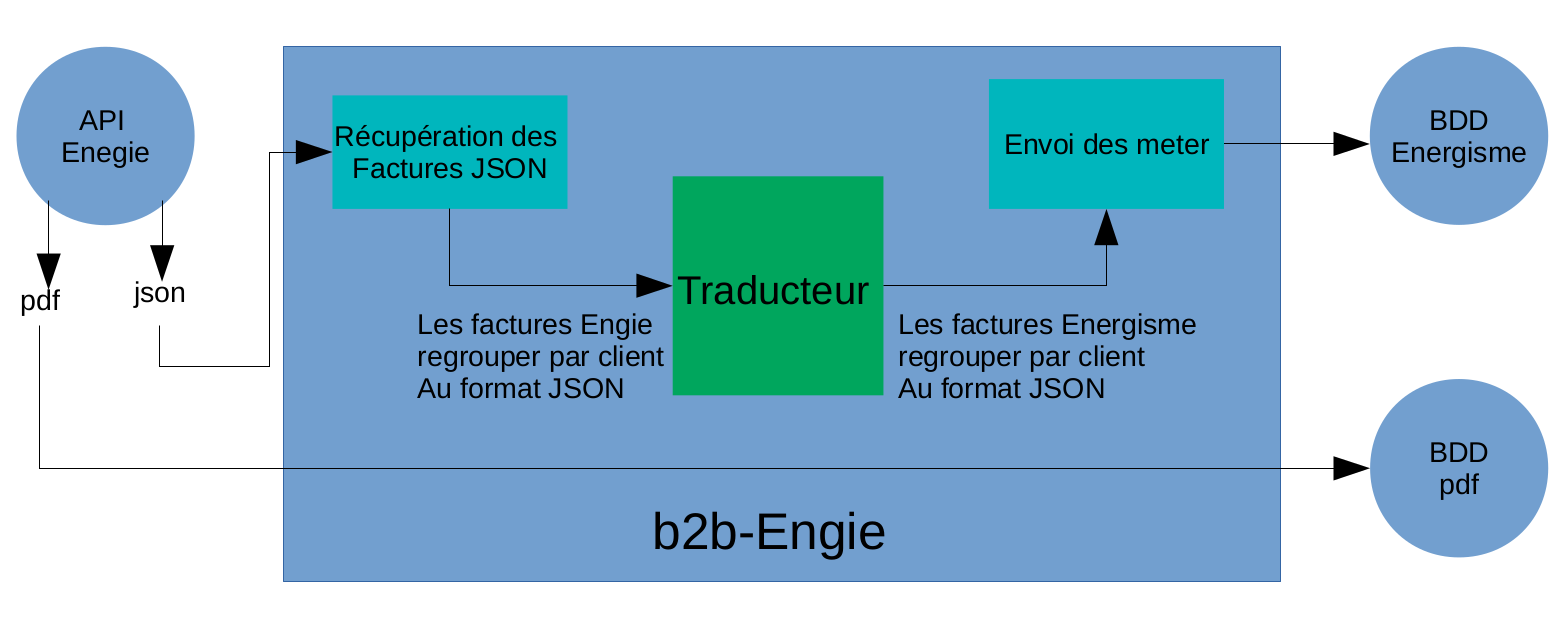
\includegraphics[scale=0.2]{14.png}
	\captionof{figure}{schéma explicatif du b2b-engie}
\end{center}
\subsubsection{Introduction}
Ce projet consiste à implémenter un traducteur des factures Engie vers des factures Energisme. Les détails nécessaires afin de réaliser le traducteur, figurent sur un ticket JIRA, qui exprime le besoin, le résultat attendu et le mapping qu'il faut faire. En gros :
\begin{itemize}
	\item Les données : les factures Engie au format JSON fourni par l'API Engie, les données fournies à notre traducteur et un répertoire qui contient plusieurs répertoires (un répertoire par partenaire). Chaque répertoire contient deux fichiers "getFactureDetails.json" et "getFactures.json", nous utilisons le "getFactureDetails.json" qui contient des milliers de factures, chaque ligne correspondant à une liste de factures pour un client.
	\begin{center}
		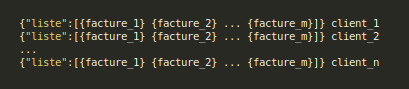
\includegraphics[scale=0.6]{18.png}
		\captionof{figure}{Exemple de fichier pour un partenaire}
	\end{center}
	\item le traducteur : notre traducteur qui va récupérer des informations de la facture Engie au format JSON et les placer dans la facture Energisme au format JSON.
	\item le résultat : les factures Energisme au format JSON. 
\end{itemize}
Ma tâche consisté à travailler sur le carré vert "le traducteur". Alors j'ai procédé de la manière suivante.
%-------------------------------------------------------------------------------------------------------------------------
\subsubsection{Implémentation}
Ce projet est constitué de deux packages :\\


\noindent\textbf{package translator :} ce module constitue le traducteur lui-même, qui est à son tour regroupe différents modules (\emph{figure 12})\\[0.5cm]
\begin{center}
	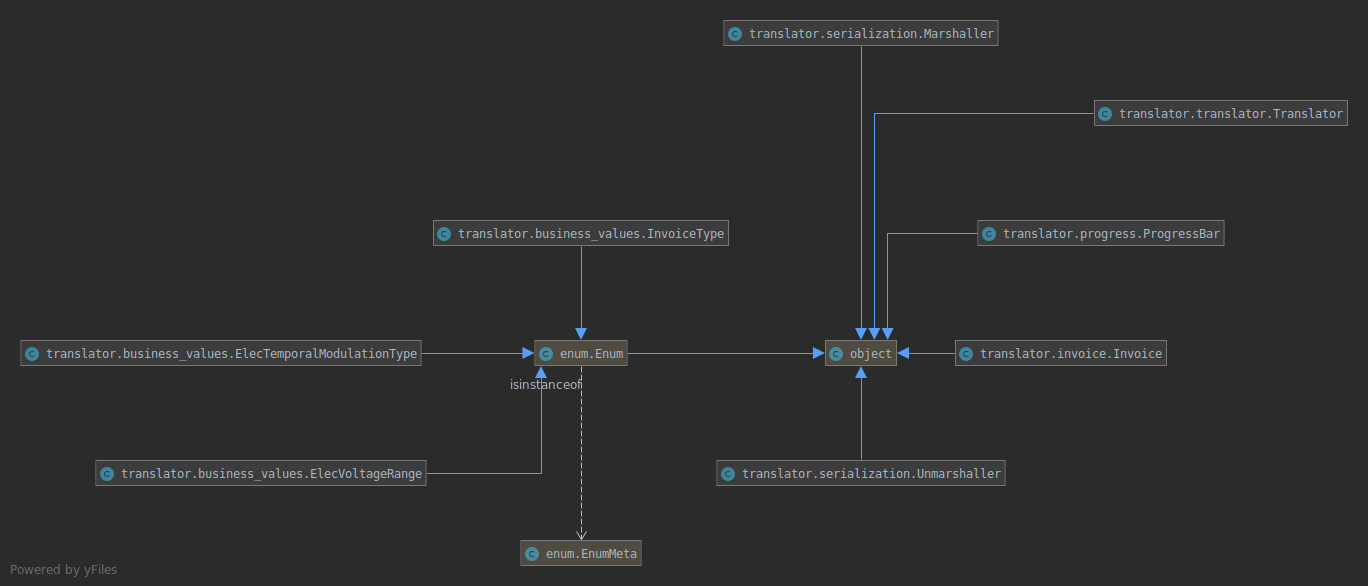
\includegraphics[scale=0.22]{16.png}
	\captionof{figure}{Architecture du package translator}
\end{center}
%========================================= main
\begin{itemize}
	\item \textbf{{\_}{\_}main{\_}{\_} :} c'est le module qui contient le programme principal qui gère les arguments d'entrée, la fonction d'usage et la fonction qui s'occupe de lire les fichiers d'entrées, appelle la classe qui fait la traduction et sauvegarder le résultat dans le répertoire de sorite.\\
	La fonction principale de ce module prend deux arguments, le répertoire source (contiens plusieurs répertoires, un par partenaire) et le répertoire de destination (un fichier par partenaire), réalise :\\
	\begin{itemize}
		\item Lire un par un et ligne par ligne le fichier "getFactureDetails.json" de chaque partenaire. 
		\item Chaque ligne est une facture, alors on fait de l'unmarshalling fichier (JSON $\to$ objet Python (dict)).
		\item On traduit l'objet python ci-dessus avec notre classe tranlator qui renvoie un autre objet (objet Python $\to$ objet Python(Invoice)).
		\item On sauvegarde tous les objets traduits du même fichier "getFactureDetails.json" dans un autre fichier qui porte comme nom "le nom du partenaire exemple : perial-normalized{\_}invoice.json" dans le dossier de destination.
	\end{itemize}  
	%========================================= serialisation
	\item \textbf{sérialisation :} ce module contient deux classes utilitaires avec plusieurs méthodes qui nous permet de sérialiser et  dé-sérialiser:
	Avec des méthodes qui acceptent de lire un fichier ou un String, d'écrire sans indentation ou avec indentation.
	\begin{itemize}
		\item "unmarshalling" : fichier JSON $\to$ objet Python.
		\item "marshalling" : objet Python $\to$ fichier JSON.  
	\end{itemize}
	%========================================= invoice
	\item \textbf{invoice :} ce module contient la classe qui représente une facture Energisme avec son format simple et les noms de clé en anglais. Cette classe contient tous les noms de clés possibles pour une facture et contient un dictionnaire qui contient la Map de clé valeur d'une instance de cette classe.
	\begin{center}
		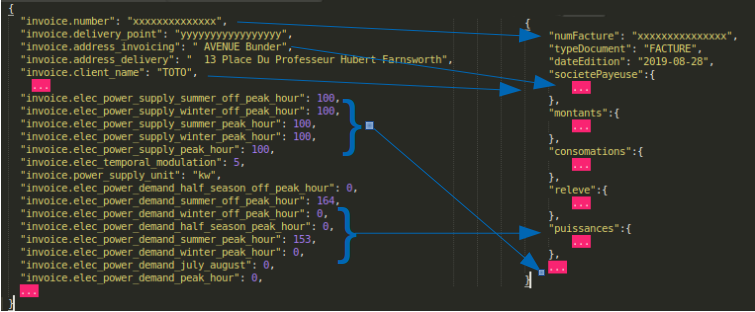
\includegraphics[scale=0.4]{17.png}
		\captionof{figure}{Petit exemple de mapping entre la facture Engie et la facture Energisme}
	\end{center} 
	%========================================= 
	\item \textbf{business{\_}values :} ce module contient tous les énumérations qui vont nous servir dans les autres module.
	%========================================= 
	\item \textbf{translator :} ce module contient la classe translator qui permet de faire la traduction. Il reçoit comme entrée une liste de factures d'un client (une ligne du fichier "getFactureDetails.json"), il va réaliser la traduction pour chaque facture de cette liste et renvoi parmi les factures traduites celle avec le plus grand nombre d'informations récupérer (le max de cette liste de factures traduite en fonction de leur longueur).\\
	Comme pour le précédent traducteur, il y a des méthodes qui renvoie une seule information, et il y a des méthodes qui retournent un ensemble d'informations (un dictionnaire clé valeur).
	\begin{center}
		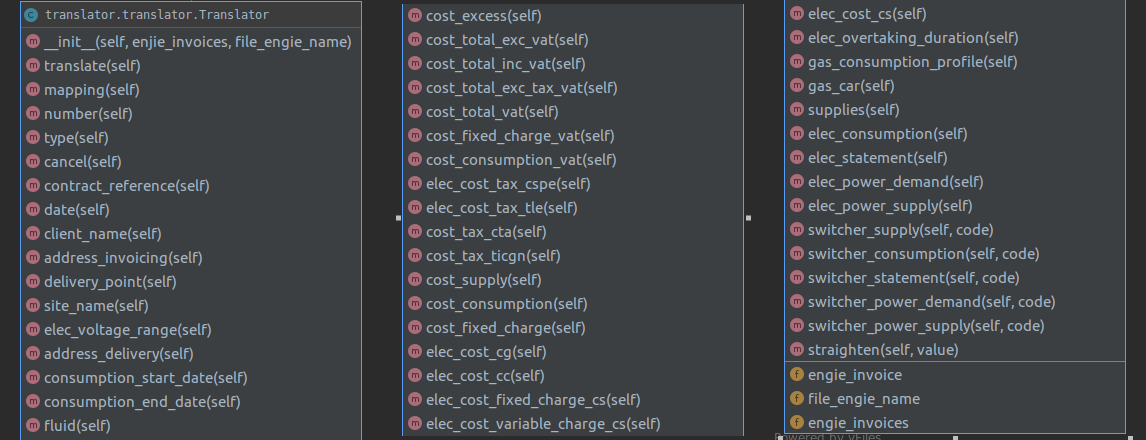
\includegraphics[scale=1.1]{19.png}
		\captionof{figure}{diagramme de classe de translator}
	\end{center} 
	%========================================= 
	\item \textbf{progress :} ce module contient une classe qui me permet d'avoir une barre de chargement quand le programme est lancé, ça me permet de savoir le temps qui reste avant la fin d’exécution.
\end{itemize}
%-------------------------------------------------------------------------------------------------------------------------
\textbf{package duplicate{\_}detector:}


Après avoir fini le projet b2b{\_}engie, il est utilisé afin de traduire les factures Engie et de produire des factures Energisme normalisés, sachant qu'il y avait déjà d’ancien factures traduites avec un autre mapping que le mien, donc cela à générer des doublons de facture dans leur base de données, il m'a donc fallu détecter et repérer ces doublons et de déterminer les différences entre ces factures afin de prendre une décision de celles qui vont être gardées et celles qui vont être supprimées.\\
Ce package fait le boulot détaillé ci-dessus, il est constitué des modules suivants :
\begin{itemize}
	\item \textbf{{\_}{\_}main{\_}{\_} :} ce module contient le programme principal qui gère les arguments d'entrée et la fonction d'usage.
	\item \textbf{detector :} ce module contient une classe qui  a un dictionnaire  qui va garder tous les factures avec une clé unique (constitué du numéro de facture standardisé sans 0 au début + id du point de livraison).\\
Pour les doublons, ils ont la même clé unique donc ils vont être ajouté dans la liste "invoices".\\
À la fin, il suffit de faire un filtre par rapport à la longueur de la liste "invoices" et on trouve tous les doublons.\\
Ce dictionnaire contient comme valeur pour chaque clé une liste de factures "invoices" la facture max, la facture min, les clés qui n'existent pas dans une facture et le plus important les valeurs différentes entre les mêmes clés.
	\begin{center}
		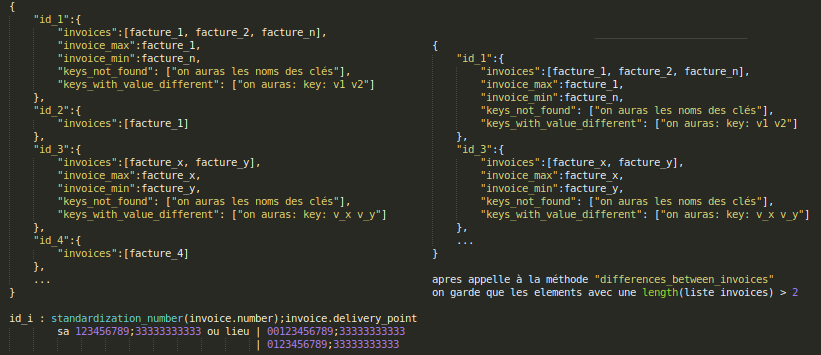
\includegraphics[scale=1.5]{21.png}
		\captionof{figure}{Représentation du detector}
	\end{center}	 
	\item \textbf{duplicate :} ce module contient les fonctions qui vont nous permettre d'avoir un système de "logging", de produire les déférents fichiers d'information et d'avoir comme résultat un répertoire par partenaire qui contient les fichiers d'informations :
	\begin{itemize}
		\item list{\_}duplicates.txt : contiens les invoice.number et le invoice.delivery{\_}point afin de supprimer les doublons après.
		\item list{\_}differences.txt : contiens les différences entre les doublons.
		\item list{\_}length.txt : contiens les longueurs des différents doublons.
	\end{itemize}
\end{itemize}    
%-------------------------------------------------------------------------------------------------------------------------
\subsubsection{Conclusion}
Je n'ai pas toujours appréhender le langage Python car je n'avais jamais codé avec, mais il s'avère qu'avec l'implémentation de ce projet, j'en ai conclu que c'est un langage de haut niveau facile à utiliser, capable de réaliser des choses complexes et sophistiqué, et cela en se basant sur peu de ligne de code.
Pour moi, ce projet m'a permis d'acquérir la maîtrise d'un nouveau langage, et d'approfondir toutes les connaissances que j'ai pu acquérir auparavant. Cette première expérience m'a permis de :
\begin{itemize}
	\item De réaliser une application python de "A" à "Z".
	\item De code avec les conventions python d’aujourd’hui.
	\item D'optimiser mon code en utilisant les lambdas expression.
	\item De réaliser une documentation et des tests unitaires pour toutes l'application. 
\end{itemize}
%-------------------------------------------------------------------------------------------------------------------------
\subsection{b2b-meter (Java)}
\subsubsection{Introduction}
Ce projet est un projet de l'entreprise déjà implémenté et utiliser, c'est un projet spring-boot, un client web service qui a comme ressource une requête post avec comme body  un objet qui contient pleine d'information :
\begin{center}
	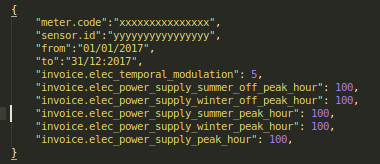
\includegraphics[scale=0.45]{22.png}
	\captionof{figure}{Exemple de l'objet injecté dans la requête post}
\end{center}
Dans cette première version, l'information est injectée dans le body de la requête (car ils n'ont pas le b2b-Enids), pour qu'à la fin, on aurait comme résultat les puissances souscrites et les puissances demandées d'une date de début à une date de fin données. Tout cela sert dans le dessin des courbes de consommations et de prédictions. Le type de requête pour cette première version :\\
"www.site.com/"load{\_}curve/{\_}search\\
Le résultat, c'est un JSON qui contient :
\begin{center}
	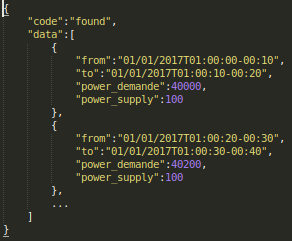
\includegraphics[scale=0.45]{23.png}
	\captionof{figure}{Exemple de résultat de la requête}
\end{center}
Ma contribution dans ce projet était de réaliser une deuxième  version plus facile à utiliser et qui récupère les puissances souscrites réelles dans les objets "meter" dont le traducteur que j'ai implémenté "b2b-Enedis" génère a priori.\\
Le type de requête pour cette deuxième version :\\
"www.site.com/"load{\_}curve/v2/\{meter.code\}/\{from\}/\{to\}\\
Le résultat, c'est un CSV qui contient :
\begin{center}
	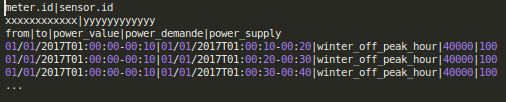
\includegraphics[scale=0.5]{24.png}
	\captionof{figure}{Exemple de résultat de la requête}
\end{center}
%-------------------------------------------------------------------------------------------------------------------------
\subsubsection{Implémentation}
Afin d'implémenter le besoin, j'ai procédé de la manier suivante, en gardant la même architecture que l'ancienne version :
\begin{itemize}
	\item Implémentation de deux client web service avec feign :
	\begin{itemize}
		\item Le premier celui qui reconnaît la requête load{\_}curve/v2/\{meter.code\}/\{from\}/\{to\}
		\begin{center}
			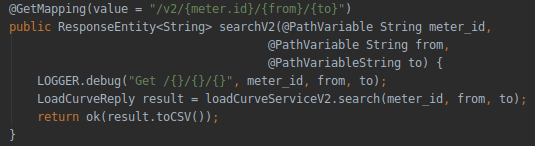
\includegraphics[scale=0.5]{28.png}
			\captionof{figure}{Exemple de client de la deuxième version de load curve.}
		\end{center}
		\item Le deuxième pour récupérer le bon "meter" dans la base de données.
		\begin{center}
			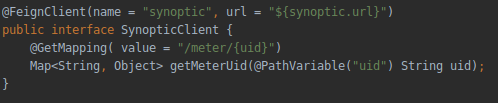
\includegraphics[scale=0.5]{27.png}
			\captionof{figure}{Interface de ce client.}
		\end{center}			
		\begin{center}
			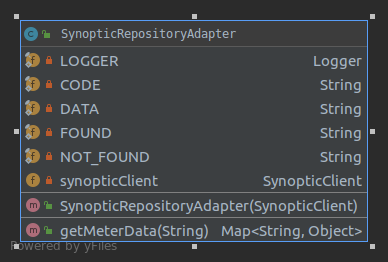
\includegraphics[scale=0.5]{29.png}
			\captionof{figure}{diagramme de classes de l'implémentation de ce client.}
		\end{center}
	\end{itemize}
	\item Implémentation de toutes les autres classes avec les modifications nécessaires. 
\end{itemize}
%-------------------------------------------------------------------------------------------------------------------------
\subsubsection{Conclusion}
Ce projet est un projet complet et professionnel déjà utilisé, donc ça m'a permis d'avoir à quoi rassemble le code d'un vrai développeur qui a plus d’expérience que moi (10 ans).
L'implémentation de ce web service m'a permis de :
\begin{itemize}
	\item Créer une application web avec Spring.
	\item Créer des clients web service avec Feign.
	\item modifier un projet déjà opérationnel, afin de faire une deuxième version. 
\end{itemize}
%-------------------------------------------------------------------------------------------------------------------------
